\section{INTRODUCTION}
\label{sec:introduction}

Whether a quantum extreme learning machine (QELM) can replace a quantum
reservoir computer (QRC) depends on more than model capacity: it depends on
access to the past. We establish when recent inputs contain enough
information to reproduce a reservoir's outputs, how much context is
required, and when persistent memory prevents replacement by any fixed
input window.

QRCs and QELMs offer two ways to process temporal data using quantum
features \cite{fujii2017harnessing,innocenti2023potential}. A QRC carries
its quantum state forward as new inputs arrive, allowing earlier events
to influence later outputs. The reset-window QELMs considered here instead
start afresh for each prediction and receive an explicit window of recent
inputs. Their memory therefore comes from the supplied data rather than a
state retained between predictions. Time-delayed QELMs demonstrate how
this approach can support time-series prediction without maintaining
quantum state throughout the input sequence \cite{kawanabe2026tdqelm}.
This makes the question of when a window can replace recurrence
practically relevant.

\begin{figure*}[t]
 \centering
 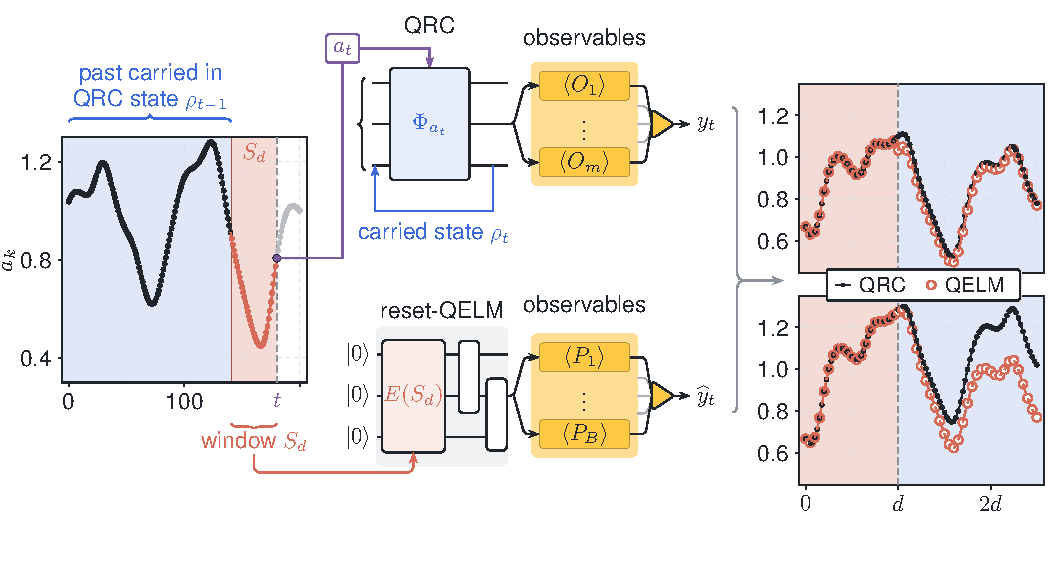
\includegraphics[width=\textwidth]{fig01_information_interface.pdf}
\caption{Two ways to provide memory: the QRC carries its quantum state
 forward, while the reset-QELM receives a window of recent inputs.
Right: an old input leaves the window at the dashed line. Above, its
influence has vanished by then, so the curves stay identical. Below, its influence
 becomes more visible and a gap remains. Orange denotes the QRC; blue
 denotes an ideal window prediction. These are schematic examples, not
 trained-model results: time advances while the window length stays fixed
 (Section~\ref{sec:models}). Here $E$ encodes the window, $O_j$ and $P_j$
 are measured observables, $m$ and $B$ count QRC outputs and QELM features,
 and $k$ indexes inputs while $t$ marks the current step.}
 \label{fig:information-interface}
\end{figure*}

The trade-off is between retaining history in a recurrent state and
supplying it explicitly through an input window. A QRC can preserve useful
information from much earlier inputs without replaying them, but its
dynamics must retain that information reliably. A reset-window QELM avoids
carrying quantum state between predictions and makes the available history
explicit, but expanding the window can require additional encoding and
processing resources. Neither approach is automatically more accurate or
more efficient: the appropriate choice depends on how much history the task
requires and the resources available to provide it.

Existing research provides complementary foundations for answering this
question. Quantum reservoir theory studies when dependence on the past
fades \cite{boyd1985fading,martinezpena2023finite}, while quantum
feature-model research establishes which functions sufficiently expressive
models can approximate \cite{goto2021universal}. We connect these
perspectives by separating two requirements: having the historical
information needed for an output, and having a representation capable of
using it.

The distinction is simple. Two input histories may have identical recent
inputs but different reservoir outputs because an earlier event still
matters. A window-only model cannot distinguish these histories, regardless
of its capacity. We quantify the resulting unavoidable error. Under our
stated assumptions and with exact expectation values, sufficiently
expressive QELMs can achieve arbitrarily accurate emulation as their windows
grow precisely when the omitted past's influence becomes uniformly
negligible across the allowed histories. We also relate the rate of
forgetting to the required context \cite{petreczky2026stability}. The
reservoir need not forget everything---only past information that can still
affect the chosen outputs matters.

Longer windows, however, do not always resolve the problem. We construct a
fixed two-qubit reservoir that performs temporal recall exactly using
expectation values. Over unbounded recall delays, every fixed-window
predictor faces the same positive worst-case error, regardless of its
capacity. This separates retained memory from finite context, rather than
quantum from classical computation.

Analytical benchmarks and simulations distinguish missing history from
limited features and finite measurements. The resulting guarantees concern
what a model can represent, not whether it can be trained efficiently or
implemented with fewer resources. Together, our results provide a practical
starting point for choosing between recurrent and window-based models:
first determine whether the available context contains the information the
task requires; then decide how best to represent and measure it.
